
%% bare_jrnl.tex
%% V1.4b
%% 2015/08/26
%% by Michael Shell
%% see http://www.michaelshell.org/
%% for current contact information.
%%
%% This is a skeleton file demonstrating the use of IEEEtran.cls
%% (requires IEEEtran.cls version 1.8b or later) with an IEEE
%% journal paper.
%%
%% Support sites:
%% http://www.michaelshell.org/tex/ieeetran/
%% http://www.ctan.org/pkg/ieeetran
%% and
%% http://www.ieee.org/

%%*************************************************************************
%% Legal Notice:
%% This code is offered as-is without any warranty either expressed or
%% implied; without even the implied warranty of MERCHANTABILITY or
%% FITNESS FOR A PARTICULAR PURPOSE! 
%% User assumes all risk.
%% In no event shall the IEEE or any contributor to this code be liable for
%% any damages or losses, including, but not limited to, incidental,
%% consequential, or any other damages, resulting from the use or misuse
%% of any information contained here.
%%
%% All comments are the opinions of their respective authors and are not
%% necessarily endorsed by the IEEE.
%%
%% This work is distributed under the LaTeX Project Public License (LPPL)
%% ( http://www.latex-project.org/ ) version 1.3, and may be freely used,
%% distributed and modified. A copy of the LPPL, version 1.3, is included
%% in the base LaTeX documentation of all distributions of LaTeX released
%% 2003/12/01 or later.
%% Retain all contribution notices and credits.
%% ** Modified files should be clearly indicated as such, including  **
%% ** renaming them and changing author support contact information. **
%%*************************************************************************


% *** Authors should verify (and, if needed, correct) their LaTeX system  ***
% *** with the testflow diagnostic prior to trusting their LaTeX platform ***
% *** with production work. The IEEE's font choices and paper sizes can   ***
% *** trigger bugs that do not appear when using other class files.       ***                          ***
% The testflow support page is at:
% http://www.michaelshell.org/tex/testflow/



\documentclass[journal]{IEEEtran}
%
% If IEEEtran.cls has not been installed into the LaTeX system files,
% manually specify the path to it like:
% \documentclass[journal]{../sty/IEEEtran}

\usepackage{algorithm}
\usepackage{algpseudocode}
\usepackage{amsmath}

\usepackage{graphicx}
\graphicspath{{img/}}




% Some very useful LaTeX packages include:
% (uncomment the ones you want to load)


% *** MISC UTILITY PACKAGES ***
%
%\usepackage{ifpdf}
% Heiko Oberdiek's ifpdf.sty is very useful if you need conditional
% compilation based on whether the output is pdf or dvi.
% usage:
% \ifpdf
%   % pdf code
% \else
%   % dvi code
% \fi
% The latest version of ifpdf.sty can be obtained from:
% http://www.ctan.org/pkg/ifpdf
% Also, note that IEEEtran.cls V1.7 and later provides a builtin
% \ifCLASSINFOpdf conditional that works the same way.
% When switching from latex to pdflatex and vice-versa, the compiler may
% have to be run twice to clear warning/error messages.






% *** CITATION PACKAGES ***
%
%\usepackage{cite}
% cite.sty was written by Donald Arseneau
% V1.6 and later of IEEEtran pre-defines the format of the cite.sty package
% \cite{} output to follow that of the IEEE. Loading the cite package will
% result in citation numbers being automatically sorted and properly
% "compressed/ranged". e.g., [1], [9], [2], [7], [5], [6] without using
% cite.sty will become [1], [2], [5]--[7], [9] using cite.sty. cite.sty's
% \cite will automatically add leading space, if needed. Use cite.sty's
% noadjust option (cite.sty V3.8 and later) if you want to turn this off
% such as if a citation ever needs to be enclosed in parenthesis.
% cite.sty is already installed on most LaTeX systems. Be sure and use
% version 5.0 (2009-03-20) and later if using hyperref.sty.
% The latest version can be obtained at:
% http://www.ctan.org/pkg/cite
% The documentation is contained in the cite.sty file itself.






% *** GRAPHICS RELATED PACKAGES ***
%
\ifCLASSINFOpdf
  % \usepackage[pdftex]{graphicx}
  % declare the path(s) where your graphic files are
  % \graphicspath{{../pdf/}{../jpeg/}}
  % and their extensions so you won't have to specify these with
  % every instance of \includegraphics
  % \DeclareGraphicsExtensions{.pdf,.jpeg,.png}
\else
  % or other class option (dvipsone, dvipdf, if not using dvips). graphicx
  % will default to the driver specified in the system graphics.cfg if no
  % driver is specified.
  % \usepackage[dvips]{graphicx}
  % declare the path(s) where your graphic files are
  % \graphicspath{{../eps/}}
  % and their extensions so you won't have to specify these with
  % every instance of \includegraphics
  % \DeclareGraphicsExtensions{.eps}
\fi
% graphicx was written by David Carlisle and Sebastian Rahtz. It is
% required if you want graphics, photos, etc. graphicx.sty is already
% installed on most LaTeX systems. The latest version and documentation
% can be obtained at: 
% http://www.ctan.org/pkg/graphicx
% Another good source of documentation is "Using Imported Graphics in
% LaTeX2e" by Keith Reckdahl which can be found at:
% http://www.ctan.org/pkg/epslatex
%
% latex, and pdflatex in dvi mode, support graphics in encapsulated
% postscript (.eps) format. pdflatex in pdf mode supports graphics
% in .pdf, .jpeg, .png and .mps (metapost) formats. Users should ensure
% that all non-photo figures use a vector format (.eps, .pdf, .mps) and
% not a bitmapped formats (.jpeg, .png). The IEEE frowns on bitmapped formats
% which can result in "jaggedy"/blurry rendering of lines and letters as
% well as large increases in file sizes.
%
% You can find documentation about the pdfTeX application at:
% http://www.tug.org/applications/pdftex





% *** MATH PACKAGES ***
%
%\usepackage{amsmath}
% A popular package from the American Mathematical Society that provides
% many useful and powerful commands for dealing with mathematics.
%
% Note that the amsmath package sets \interdisplaylinepenalty to 10000
% thus preventing page breaks from occurring within multiline equations. Use:
%\interdisplaylinepenalty=2500
% after loading amsmath to restore such page breaks as IEEEtran.cls normally
% does. amsmath.sty is already installed on most LaTeX systems. The latest
% version and documentation can be obtained at:
% http://www.ctan.org/pkg/amsmath





% *** SPECIALIZED LIST PACKAGES ***
%
%\usepackage{algorithmic}
% algorithmic.sty was written by Peter Williams and Rogerio Brito.
% This package provides an algorithmic environment fo describing algorithms.
% You can use the algorithmic environment in-text or within a figure
% environment to provide for a floating algorithm. Do NOT use the algorithm
% floating environment provided by algorithm.sty (by the same authors) or
% algorithm2e.sty (by Christophe Fiorio) as the IEEE does not use dedicated
% algorithm float types and packages that provide these will not provide
% correct IEEE style captions. The latest version and documentation of
% algorithmic.sty can be obtained at:
% http://www.ctan.org/pkg/algorithms
% Also of interest may be the (relatively newer and more customizable)
% algorithmicx.sty package by Szasz Janos:
% http://www.ctan.org/pkg/algorithmicx




% *** ALIGNMENT PACKAGES ***
%
%\usepackage{array}
% Frank Mittelbach's and David Carlisle's array.sty patches and improves
% the standard LaTeX2e array and tabular environments to provide better
% appearance and additional user controls. As the default LaTeX2e table
% generation code is lacking to the point of almost being broken with
% respect to the quality of the end results, all users are strongly
% advised to use an enhanced (at the very least that provided by array.sty)
% set of table tools. array.sty is already installed on most systems. The
% latest version and documentation can be obtained at:
% http://www.ctan.org/pkg/array


% IEEEtran contains the IEEEeqnarray family of commands that can be used to
% generate multiline equations as well as matrices, tables, etc., of high
% quality.




% *** SUBFIGURE PACKAGES ***
%\ifCLASSOPTIONcompsoc
%  \usepackage[caption=false,font=normalsize,labelfont=sf,textfont=sf]{subfig}
%\else
%  \usepackage[caption=false,font=footnotesize]{subfig}
%\fi
% subfig.sty, written by Steven Douglas Cochran, is the modern replacement
% for subfigure.sty, the latter of which is no longer maintained and is
% incompatible with some LaTeX packages including fixltx2e. However,
% subfig.sty requires and automatically loads Axel Sommerfeldt's caption.sty
% which will override IEEEtran.cls' handling of captions and this will result
% in non-IEEE style figure/table captions. To prevent this problem, be sure
% and invoke subfig.sty's "caption=false" package option (available since
% subfig.sty version 1.3, 2005/06/28) as this is will preserve IEEEtran.cls
% handling of captions.
% Note that the Computer Society format requires a larger sans serif font
% than the serif footnote size font used in traditional IEEE formatting
% and thus the need to invoke different subfig.sty package options depending
% on whether compsoc mode has been enabled.
%
% The latest version and documentation of subfig.sty can be obtained at:
% http://www.ctan.org/pkg/subfig




% *** FLOAT PACKAGES ***
%
%\usepackage{fixltx2e}
% fixltx2e, the successor to the earlier fix2col.sty, was written by
% Frank Mittelbach and David Carlisle. This package corrects a few problems
% in the LaTeX2e kernel, the most notable of which is that in current
% LaTeX2e releases, the ordering of single and double column floats is not
% guaranteed to be preserved. Thus, an unpatched LaTeX2e can allow a
% single column figure to be placed prior to an earlier double column
% figure.
% Be aware that LaTeX2e kernels dated 2015 and later have fixltx2e.sty's
% corrections already built into the system in which case a warning will
% be issued if an attempt is made to load fixltx2e.sty as it is no longer
% needed.
% The latest version and documentation can be found at:
% http://www.ctan.org/pkg/fixltx2e


%\usepackage{stfloats}
% stfloats.sty was written by Sigitas Tolusis. This package gives LaTeX2e
% the ability to do double column floats at the bottom of the page as well
% as the top. (e.g., "\begin{figure*}[!b]" is not normally possible in
% LaTeX2e). It also provides a command:
%\fnbelowfloat
% to enable the placement of footnotes below bottom floats (the standard
% LaTeX2e kernel puts them above bottom floats). This is an invasive package
% which rewrites many portions of the LaTeX2e float routines. It may not work
% with other packages that modify the LaTeX2e float routines. The latest
% version and documentation can be obtained at:
% http://www.ctan.org/pkg/stfloats
% Do not use the stfloats baselinefloat ability as the IEEE does not allow
% \baselineskip to stretch. Authors submitting work to the IEEE should note
% that the IEEE rarely uses double column equations and that authors should try
% to avoid such use. Do not be tempted to use the cuted.sty or midfloat.sty
% packages (also by Sigitas Tolusis) as the IEEE does not format its papers in
% such ways.
% Do not attempt to use stfloats with fixltx2e as they are incompatible.
% Instead, use Morten Hogholm'a dblfloatfix which combines the features
% of both fixltx2e and stfloats:
%
% \usepackage{dblfloatfix}
% The latest version can be found at:
% http://www.ctan.org/pkg/dblfloatfix




%\ifCLASSOPTIONcaptionsoff
%  \usepackage[nomarkers]{endfloat}
% \let\MYoriglatexcaption\caption
% \renewcommand{\caption}[2][\relax]{\MYoriglatexcaption[#2]{#2}}
%\fi
% endfloat.sty was written by James Darrell McCauley, Jeff Goldberg and 
% Axel Sommerfeldt. This package may be useful when used in conjunction with 
% IEEEtran.cls'  captionsoff option. Some IEEE journals/societies require that
% submissions have lists of figures/tables at the end of the paper and that
% figures/tables without any captions are placed on a page by themselves at
% the end of the document. If needed, the draftcls IEEEtran class option or
% \CLASSINPUTbaselinestretch interface can be used to increase the line
% spacing as well. Be sure and use the nomarkers option of endfloat to
% prevent endfloat from "marking" where the figures would have been placed
% in the text. The two hack lines of code above are a slight modification of
% that suggested by in the endfloat docs (section 8.4.1) to ensure that
% the full captions always appear in the list of figures/tables - even if
% the user used the short optional argument of \caption[]{}.
% IEEE papers do not typically make use of \caption[]'s optional argument,
% so this should not be an issue. A similar trick can be used to disable
% captions of packages such as subfig.sty that lack options to turn off
% the subcaptions:
% For subfig.sty:
% \let\MYorigsubfloat\subfloat
% \renewcommand{\subfloat}[2][\relax]{\MYorigsubfloat[]{#2}}
% However, the above trick will not work if both optional arguments of
% the \subfloat command are used. Furthermore, there needs to be a
% description of each subfigure *somewhere* and endfloat does not add
% subfigure captions to its list of figures. Thus, the best approach is to
% avoid the use of subfigure captions (many IEEE journals avoid them anyway)
% and instead reference/explain all the subfigures within the main caption.
% The latest version of endfloat.sty and its documentation can obtained at:
% http://www.ctan.org/pkg/endfloat
%
% The IEEEtran \ifCLASSOPTIONcaptionsoff conditional can also be used
% later in the document, say, to conditionally put the References on a 
% page by themselves.




% *** PDF, URL AND HYPERLINK PACKAGES ***
%
%\usepackage{url}
% url.sty was written by Donald Arseneau. It provides better support for
% handling and breaking URLs. url.sty is already installed on most LaTeX
% systems. The latest version and documentation can be obtained at:
% http://www.ctan.org/pkg/url
% Basically, \url{my_url_here}.




% *** Do not adjust lengths that control margins, column widths, etc. ***
% *** Do not use packages that alter fonts (such as pslatex).         ***
% There should be no need to do such things with IEEEtran.cls V1.6 and later.
% (Unless specifically asked to do so by the journal or conference you plan
% to submit to, of course. )


% correct bad hyphenation here
\hyphenation{op-tical net-works semi-conduc-tor}


\begin{document}
%
% paper title
% Titles are generally capitalized except for words such as a, an, and, as,
% at, but, by, for, in, nor, of, on, or, the, to and up, which are usually
% not capitalized unless they are the first or last word of the title.
% Linebreaks \\ can be used within to get better formatting as desired.
% Do not put math or special symbols in the title.
\title{More surface detail with\\ One-Two-Pixel Matching}
%
%
% author names and IEEE memberships
% note positions of commas and nonbreaking spaces ( ~ ) LaTeX will not break
% a structure at a ~ so this keeps an author's name from being broken across
% two lines.
% use \thanks{} to gain access to the first footnote area
% a separate \thanks must be used for each paragraph as LaTeX2e's \thanks
% was not built to handle multiple paragraphs
%Y. Qin and C. Mallet are with the MATIS, Université Paris-Est, IGN, 94160

\author{Ewelina~Rupnik 
        and Marc~Pierrot~Deseilligny,% <-this % stops a space
\thanks{E. Rupnik and M. Pierrot Deseilligny are with LASTIG IGN, ENSG, Universite Paris-Est, 94160 Saint-Mandé, France}% <-this % stops a space 
\thanks{Manuscript received April 19, 2005; revised August 26, 2015.}}

% note the % following the last \IEEEmembership and also \thanks - 
% these prevent an unwanted space from occurring between the last author name
% and the end of the author line. i.e., if you had this:
% 
% \author{....lastname \thanks{...} \thanks{...} }
%                     ^------------^------------^----Do not want these spaces!
%
% a space would be appended to the last name and could cause every name on that
% line to be shifted left slightly. This is one of those "LaTeX things". For
% instance, "\textbf{A} \textbf{B}" will typeset as "A B" not "AB". To get
% "AB" then you have to do: "\textbf{A}\textbf{B}"
% \thanks is no different in this regard, so shield the last } of each \thanks
% that ends a line with a % and do not let a space in before the next \thanks.
% Spaces after \IEEEmembership other than the last one are OK (and needed) as
% you are supposed to have spaces between the names. For what it is worth,
% this is a minor point as most people would not even notice if the said evil
% space somehow managed to creep in.



% The paper headers
\markboth{Journal of \LaTeX\ Class Files,~Vol.~14, No.~8, August~2015}%
{Shell \MakeLowercase{\textit{et al.}}: Even more detail with One-Two-Pixel Matching}
% The only time the second header will appear is for the odd numbered pages
% after the title page when using the twoside option.
% 
% *** Note that you probably will NOT want to include the author's ***
% *** name in the headers of peer review papers.                   ***
% You can use \ifCLASSOPTIONpeerreview for conditional compilation here if
% you desire.




% If you want to put a publisher's ID mark on the page you can do it like
% this:
%\IEEEpubid{0000--0000/00\$00.00~\copyright~2015 IEEE}
% Remember, if you use this you must call \IEEEpubidadjcol in the second
% column for its text to clear the IEEEpubid mark.



% use for special paper notices
%\IEEEspecialpapernotice{(Invited Paper)}




% make the title area
\maketitle

% As a general rule, do not put math, special symbols or citations
% in the abstract or keywords.
\begin{abstract}
Photogrammetrically derived Digital Surface Models have been widely adopted in geoscientific applications such us mapping and change detection across volcanic surfaces, glaciers, areas of seismic activity, forests, river landforms etc.  Resolution of the reconstructed surface is crucial as more accurate information allows for more profound understanding of the phenomena. With this objective in mind, the research presented here proposes a new matching cost function that produces surfaces of enhanced resolution with respect to the golden standard, window-based semi-global matching technique. {We evaluate the algorithm on different image datasets spanning various acquisition geometries, radiometric qualities and GSD sizes. In particular, results on Earth satellites (SPOT-7, Pl\'eiades), extraterrestrial (Chang'E3 moon landing), aerial and UAV acquisitions are shown}. The implementation of the method is available in the free open-source software for photogrammetry -- MicMac.
 

\end{abstract}

% Note that keywords are not normally used for peerreview papers.
\begin{IEEEkeywords}
dense image matching; multi-view; forestry, bare soil, urban area; 
\end{IEEEkeywords}






% For peer review papers, you can put extra information on the cover
% page as needed:
% \ifCLASSOPTIONpeerreview
% \begin{center} \bfseries EDICS Category: 3-BBND \end{center}
% \fi
%
% For peerreview papers, this IEEEtran command inserts a page break and
% creates the second title. It will be ignored for other modes.
\IEEEpeerreviewmaketitle



\section{Introduction}
% 
% 
% Here we have the typical use of a "T" for an initial drop letter
% and "HIS" in caps to complete the first word.
\IEEEPARstart{T}{e} dense image matching for digital surface model (\textit{DSM} or \textit{photogrammetric DSM}) generation has been an accepted method across the geoscience communities. Next to other competitive techniques such as \textit{LiDAR} or radar, image-based reconstruction produces denser 3D information, is richer as it includes the photometric observations allowing for e.g. 3D change detection or classification, and is cost effective. %Nonetheless, imaging in the optical spectrum means dependency on the meteorological conditions, the Sun, as well as 3D results subject to noise and the presence of outliers.\par 
%apps
Photogrammetric DSMs in geoscience applications can be generated from terrestrial images, UAV acquisitions or high-resolution optical satellite imaging. 
%terrestrial UAV apps
\paragraph{Terrestrial and UAV applications}
%Photogrammetry at close range has the advantage with respect to other methods (e.g. contact profilometers) in that it is not invasive, the measurements are done remotely, capture the surface at one instance and with many samples. 
Modelling of surface roughness parameters  \cite{bretar2013advanced}; mapping volcanic surfaces \cite{kolzenburg2016rapid}; measuring glaciar's microrelief progression~\cite{kaab2014surface} are among examples of terrestrial applications carried out with consumer grade camera and little expert knowledge.
%
% \cite{bretar2013advanced} showed that photogrammetric DSMs generated from hand acquisitions by a DSLR camera can be used to extract surface roughness parameters. From these local DSMs one can then infer roughness parameters over large-scale areas and complete the lower-resolution data provided by other sensors (e.g. InSAR). \cite{kolzenburg2016rapid} sees a great potential in photogrammetry to perform frequent updating at high spatial resolution of volcanic surfaces, that could e.g. serve to help understand the dynamic processes such as lava-flow emplacements or cinder cones growth.\par 
%
UAV-based surveys are increasingly present as an alternative to terrestrial surveys due to their larger reach, the ease of employment and little operational cost. Resolution-wise, it is a compromise between high-resolution close-range and moderate-resolution satellite imaging. The success of the UAV technology is reflected in numerous publications where, e.g., UAV-collected imagery enables modelling of the forest canopy height \cite{lisein2013photogrammetric}; determines the rate and extent of landslide movements \cite{niethammer2010uav}; in aeolian research quantifies coastal erosion \cite{d2012unmanned}, \cite{james2012straightforward} and deposition processes \cite{hugenholtz2013geomorphological}; in tectonic research maps ultrafine (i.e. centimetric) tectonic faults \cite{johnson2014rapid}; or in glaciology is employed in repeated surveys of the ice-sheet masses \cite{ryan2015uav}.


%\cite{niethammer2010uav} adopted a UAV platform to determine the rate and extent of landslide movements. In the same vein, \cite{hugenholtz2013geomorphological} makes use of UAV and photogrammetry in aeolian research. Accurate DSMs permit to quantify a landscape's erosion and deposition processes. \cite{johnson2014rapid} validates the suitability of photogrammetric DSMs in mapping ultrafine (i.e. centimetric) tectonic faults. \cite{ryan2015uav} applied repeated UAV surveys to study the change of a Greenland glacier's volume across a two-month period. In the vulnerable coastal zones of Marocco \cite{d2012unmanned} examines the soil erosion achieving decentimetric accuracies. Likewise, \cite{james2012straightforward} create spatiotemporal erosion maps of coastal erosion and disclose its retreat rate with unprecedented precision.
 
%more on ladnslide -- sajidd paper 

% James and Robson (2012) -- cliff erosion
%Rosnell and Honkavaara, 2012
%Fonstad et al., 2013
 

%%%%%%%%%Satellites apps + about MARS!!!
%+bare soil (tecto + roughness)
%+forest
%+urban zones?
%extraterrestrial
\paragraph{Earth satellite and extraterrestrial applications}
With the available optical satellite data provided by modern (e.g. Pl\'eiades~1A/B, SPOT-satellites, QuickBird, WorldView~2/3/4, CubeSat) or the older generation satellites (e.g. CartoSat, ASTER) we can capture the Earth surface at Ground Sampling Distances (GSD) in the range of a few m~--~0.3m, yielding DSMs of similar resolution \cite{rupnik:17:fusion}. Coupled with the daily revisit times, the satellite images are a suitable tool for mapping the surface evolution. To take a few \textit{state-of-the-art} examples, satellite images are used to: identify patterns and rates of sand dunes migrations \cite{hermas2012retrieving}; quantify post-seismic surface displacements \cite{rosu2015measurement}, \cite{vallage2015inelastic}; estimate timber volume in a densely forested area \cite{straub2013assessment}; study the time-varying coastal shelf \cite{tseng2017reconstruction}; employ multi-temporal DSMs for elevation change studies across glaciers, volcanoes and river landforms \cite{girod2017mmaster}; or map other planet's topographies \cite{gwinner2010topography}.\par 
%
In all of the mentioned applications resolution of the surface plays a significant role because it improves the observability of the phenomena. Following the principle that if one can see more detail, to the same degree one can more easily spot a small detail change, an image matching algorithm that furnishes better  resolution surfaces renders possible change detection at finer-level detail. Put differently, it allows for earlier change detection. The research presented in this publication addresses fine resolution surface reconstruction by proposing a novel image matching technique. 

%the importance of fidelity of reconstruction, precision _you'll need to get back to all papers
% \cite{johnson2014rapid} gridding artefacts at low resolution dsms

%+motivation that we keep the footprint big and increase the resolution of the output  
 
 
%RYAN
%Despite significant advances in satellite remote sensing, limitations of spatial resolution (e.g. MODIS) and/or frequency of repeat imagery (e.g. Landsat or TerraSar-X) render de-tailed, day-to-day analysis of calving-front dynamics un- feasible. On the other hand, acquisition of digital imagery from un
 
 

\subsection{Related work}
\paragraph{Generalities}
Photogrammtrically derived DSMs are typically found by solving an energy functional with {global}, semi-global (SGM) or local methods.\par  
Classically, local methods calculate the best correspondences in three steps: (i) matching cost calculation, (ii) support domain cost aggregation, and (iii) the depth selection by the \textit{Winner-Takes-All}  \cite{yoon2005locally}, or the belief propagation schemes \cite{bleyer2011patchmatch,galliani2015massively}. The local character of the methods makes them computationally efficient, often at the expense of lower 3D precision and completeness.\par 
%
Whether global or SGM approach, the best correspondences are found by minimizing a cost function that is a sum of the data and the regularity term. Global methods minimize the energy defined over all pixels in a MRF graph with techniques such as $\alpha$-expansion moves \cite{boykov2001fast,taniai2017continuous} or message passing \cite{felzenszwalb2006efficient}. Alternatively, definition over a continuous space and sub-pixelar reconstruction precision is is possible with variational methods \cite{ranftl2012pushing}. Such minimization is NP-hard, and does not allow for concave regularity terms. The first poses memory issues for large scale reconstructions, while the latter inhibits faithful reconstruction at discontinuities (e.g. buildings). \par 
%
The SGM methods are solved with multi-directional dynamic programming techniques, impose no constraint on the regularity term and the optimization is resolved along independent lines of pixels \cite{mpd:06:sgm,hirschmuller:08:sgm}. Therefore, the computational times remain reasonable as the image size grows. Since cost function is cumulative along a number of directions, the found optimal solution is close to the global solution. \par 
%
 

\paragraph{Matching cost calculation}
Independently of the algorithm, there exist many different measures to describe the similarity (i.e. \textit{photo-consistency}) between pixel correspondences. The very first and most straightforward measure compares the pixel intensity values \cite{kanade1995development,birchfield1998pixel}. In real-world conditions (i.e. non-Lambertian surfaces, radiometric differences due to illumination change), in the presence of non-textures zones or repetitive patterns, however, pixel intensity differences turn to be unreliable for matching. In practice, photo-consistency measures defined over a support domain (square windows ordinarily of   $3 x 3$, $5 x 5$, etc. size) are preferred \cite{furukawa2015multi}, e.g. zero-mean normalized cross-correlation (NCC), Census, Rank \cite{zabih1994non}, Mutual Information \cite{viola1997alignment}. Including more context within the per-pixel matching is advantageous for it increases the uniqueness and the robustness of the matched points, as well as attenuates the noise (caused by the low signal-to-noise ratio of the sensor). Note, however, that (i) it interpolates the image signal within the support and possibly misses the surface fine structures, as well as (ii) a pixel-wise cost aggregated over a support window assumes constant disparity within the aggregated neighbourhood. The latter results in smoothness artefacts or mismatches if it happens to overlap a discontinuity, e.g. a building's edge. Furthermore, if the support window is chosen to be a square region, it takes for granted that the square shape in one view will project to an exact square in another view. Therefore, the perspective transformation the shape undergoes once projected to 3D and subsequently back-projected to another view, are neglected (the so-called \textit{window foreshortening} problem).\par 
%
Numerous approaches have been proposed to overcome the above shortcomings. To mitigate the mismatches at discontinuities adaptive support windows avoiding discontinuities \cite{yoon2006adaptive}, adaptive windows minimising a cost, or intensity gradient cost aggregation \cite{hirschmuller:08:sgm} were proposed.
 Sweeping-planes \cite{gallup2007real}, 3D slanted windows \cite{bleyer2011patchmatch}, or a fusion of a slanted and adaptive windows (i.e. elongated windows with different orientations) \cite{buades2015reliable} were adopted to account for different surface slopes. Initialisation of the surface planes is carried out by analysing the sparse reconstruction \cite{gallup2007real}, dense reconstruction computed with square windows  \cite{yoon2006adaptive} or by random assignment \cite{bleyer2011patchmatch}. Each choice comes with a certain risk of missing the correct surface slope or providing incomplete initialisation. For instance, sparse reconstruction can initialize only in places where 3D points exist hence omits poorly textured areas, classical dense reconstruction may fail at providing good initial surfaces at discontinuities and slopes, whereas random selection gives no guarantee of assigning the suitable plane slope to either of the pixels belonging to a region underlying that plane. \\
%



\subsection{Contributions}
In this work we aim at {enhanced precision depth} reconstruction free from   {fronto-parallel artefacts} and with good performance at {surface discontinuities}. To realise it we:%add large baseline?

\begin{itemize}
\item[--] formulate a new matching cost defined over a single pixel,
\item[--] adopt a second pixel to allow for slope testing with minimum information (a slope is defined by two points in 3D space and it is tested with exactly two pixels),
\item[--] embed the image dense matching in a semi-global matching framework which favours slope coherence in the neighbourhood of a point and ensures surface continuity in poorly textured areas. 
\end{itemize}
%we formulate a new matching cost defined over a single pixel. By adopting a second pixel we allow for slope testing with minimum information (a slope is defined by two points in 3D space which we test with exactly two pixels). Moreover, we embed the image dense matching in a semi-global matching framework which ensures continuity   
To increase the robustness of the reconstruction the matching cost is defined in a multi-view constraint. 
 
 
%Accordingly, the proposed One-Two-Pixel matching is embedded in a SGM optimization framework and the increased precision is accomplished by formulating:
%\begin{itemize}
%\item[--] a robust one pixel multi-view photo-consistency measure, and
%\item[--] an additional two pixel term.
%\end{itemize}
%

\section{Methods}
%
% present it first in a 2-view and then n-view config; adopt the latest graphics from pres to multiview
%about testing the slope in fact
\subsection{One-Two-Pixel cost function}
% as in cfpt but including all normalisation
%generalities
With the objective of excelling the spatial resolution of reconstructed depths, we propose a reformulated energy functional (\ref{eq:sgmOnePix}):\par 
%


\begin{figure}[h]
\begin{equation}\label{eq:sgmOnePix}       
\begin{split}          
  \mathcal C (D) = \sum_{p=1}^N  C^I(p,d_p) +  \\
                   \sum_{q=Np} C^C(\mathbf{d_p},\mathbf{d_q}) + \sum_{q=Np} C^T(\mathbf{d_p},\mathbf{d_q}) 
\end{split}                  
\end{equation}
\end{figure}
% 
where $C^I$ is the single-pixel term, $C^C$ is the two-pixel term, $C^T$ is the smoothing term, $N$ is the number of all pixels, $d_p$ is a disparity at position $p$ and $d_q$ is the disparity at position $q$ belonging to $N_p$ neighbourhood of $p$. $\mathcal C (D)$ is the minimum cost of assigning the optimal depths  $ \mathcal D$ across all pixels.  The minimum solution is found in the following three steps: cost assignment (see Alg.~\ref{alg:costPix}), cost aggregation (see Alg.~\ref{alg:costAggreg}) and the optimal depth selection. The described methods are implemented in MicMac -- the free open-source software for photogrammetry \cite{rupnik2017micmac}.\par 
%
\paragraph{Two-pixel data term}
%
$C^C$ encodes the dissimilarity of a two-pixel window across multiple views ($NbV$), see~Eq.~\eqref{eq:crois}. Ideally, the advantages of the minimum window are twofold: (i) it is more apt to reconstruct fine 3D scene structure than the usual square correlation window, and (ii) is less susceptible to noisy data than as if only the single pixel term was used.

Employing the $C^C$ is equivalent of iterating over $\mathbf{d_q}$ and verifying the coherency of a given slope with the image data, the final cost of a slope assignment being an accumulation of the dissimilarities calculated independently for each stereo pair.  Speaking in terms of the cost structure, the $C^C$ costs associate with the arcs (in analogy to $C^T$), rather than with the nodes as is the case of $C^I$ (see Alg.~\ref{alg:costAggreg} and Fig.~\ref{fig:costCubeStereo}). Note that the two-pixel term should not be confused with the smoothness term. The latter applies "blind" penalization, without considering the pixel intensity values.

For a depth assignment $d_p$, the $C^C$ cost will depend on the differences of normalised intensity ratios at position $p$ and $q$. The choice of ratios was made to guarantee a robust comparison in the presence of additive and multiplicative illumination changes across the views.  The role of $Pds_{C}$ is to control the relative influence of the $C^C$ term in the cost function. In  all our tests it was also set to $1.0$.   
%
%The philosophy behind the two-pixel term 
\begin{figure}[H]
\begin{equation}\label{eq:crois}
C^C({d_p},{d_q}) = Pds_{C} \cdot \frac{1}{NbV-1}  \cdot  \sum_{v=1}^{NbV-1} \left[ \frac{I_{d_p}^v}{I_{d_p}^0} - \frac{I_{d_q}^v}{I_{d_q}^0} \right]
\end{equation}
\end{figure} 
%\\
%
\paragraph{Single-pixel data term}
%
$C^I$ is the cost of assigning a particular depth to the position $p$. It is implemented as a truly one-pixel measure and conveys the dissimilarity of two pixels in multiple views ($NbV$), see  Eq.~(\ref{eq:cost}). To match the dynamic range of the \textit{two-pixel} term, it is expressed as a mean of all intensity ratios between the master $I_0$ and the slaves $I_v$. The $\delta_v$ parameter is added to model the view-dependent radiometric differences that may disturb the cumulative cost (this is unlike in the $C^C$ expression where the effect of the radiometry change is fully modelled by the difference of ratios). The value of the parameter is  a function of intensity ratios between the master image and a slave image. It can be pixel-dependent -- if non-constant radiometric corrections across the images are necessary (e.g. specular reflections) -- or take a global value per an image (see Alg.~\ref{alg:costPix} where $\delta_v$ is computed on the pixel basis). When a pixel-dependent case is chosen, the ratios shall be first smoothed by simple averaging or by 2D polynomial function fit. 

$Pds_{I}$ is a weighting factor and it plays the same role as $Pds_{C}$. In all our tests we set the value to 1.0.\par 
%
\paragraph{Regularizing term}
%draw the regul
? do we want to talk about it?
%
%new single pixel cost function
%
\begin{figure}[H]
\begin{equation}\label{eq:cost}
C^I(p,d_p) = Pds_{I} \cdot \frac{1}{NbV-1} \cdot \sum_{v=1}^{NbV-1} \cdot \delta_v \cdot \left[ 1 - \frac{I_{d_p}^v}{I_{d_p}^0} \right]
\end{equation}
\end{figure}
%
\begin{figure}[h]
\centering
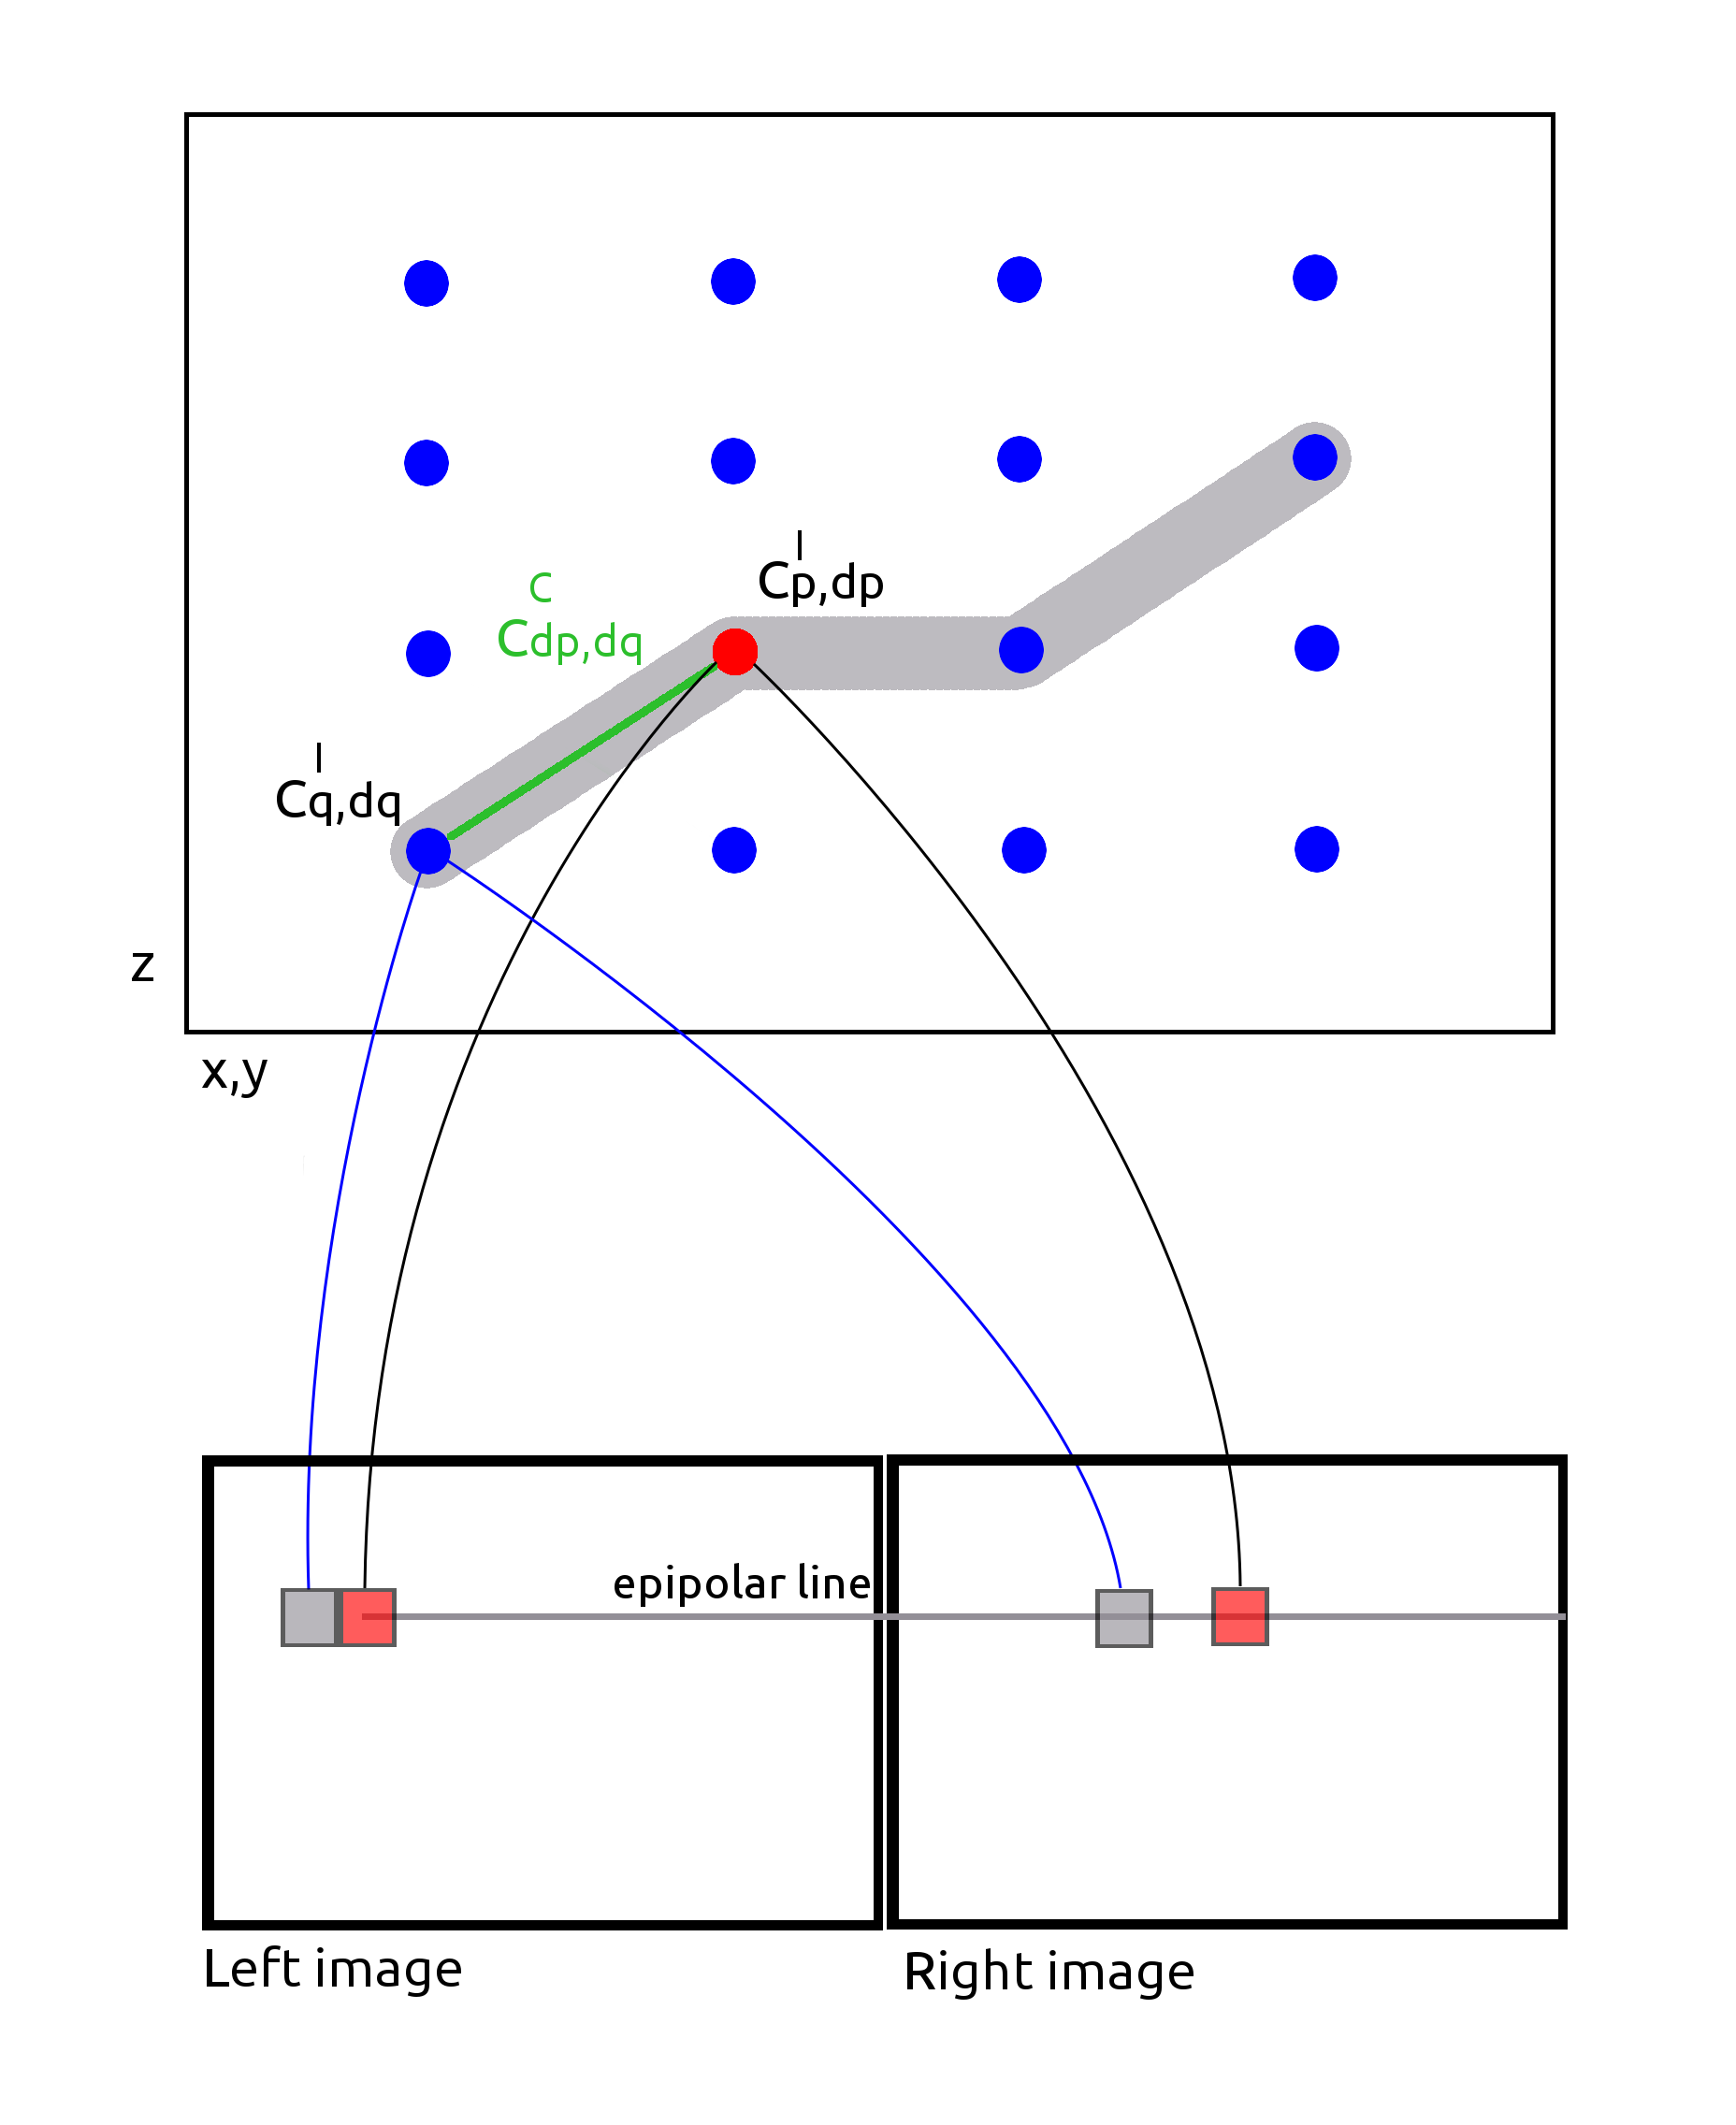
\includegraphics[width=0.4\textwidth]{cost_12Pix-2-v5.png} \caption{\textit{Top: One-two-Pixel cost structure corresponding to a stereo pair. In grey is the surface to be inferred from the matching. $C^I_{p,dp}$ and $C^I_{q,dq}$ are the costs of taking disparity $dp$ at $p$ and $dq$ at $q$ , respectively. $C^C_{dp,dp}$ is the cost of assigning a given slope. Bottom: A stereo pair that feeds the cost structure. The cost structure is illustrated on a stereo pair in epipolar geometry, however, the implemented algorithm is not constrained by the number of views and, by default, operates in the original image geometry.}}\label{fig:costCubeStereo}
\end{figure}
% 
\begin{algorithm}
\caption{Cost assignment}
\begin{algorithmic}
\State  $VIm[v].ImOrth(X,Y)$ - intensity in image $v$ at position $(X,Y)$; all images are orthorectified to the geometry of the master\\
\State  $ratio(int,int)$ - calculate ratios
\State  $norm(int)$ - normalise to [0-255]
\State  $\delta$ - radiometric calibration
\State  $SurfOpt$ - optimiser\\

\Comment {Assignment}
\For {$Z=Z_{min}; Z<Z_{max}; Z++$} 
\For {$X=0; X<Sz.x; X++$} 
\For {$Y=0; Y<Sz.y; Y++$} \\

\State $V_0=VIm[0].ImOrth(X,Y)$
\State $C^I=0$
\For {$v=0; v<NbV; v++$} \\
\State $V_k=VIm[v].ImOrth(X,Y)$
\State $Val=ratio(V_0,V_k)$
\State $Val=norm(Val)$
\State $r.push\_back( Val )$\\

\State $V_k^{cor} = \delta_v V_k$
\State $Val^{cor} = ratio(V_0,V_k^{cor})$
\State $C^I+=Abs(Val^{cor})$ 
\EndFor \\
\\
\Comment {Communicate the vector of ratios and the data term to the optimiser}
\State  $ SurfOpt(X,Y,Z) = r $
\State  $ SurfOpt(X,Y,Z) = C^I$ \\

\EndFor
\EndFor 
\EndFor  

\end{algorithmic}\label{alg:costPix}
\end{algorithm}
%
% 
\begin{algorithm*}
\caption{Cost aggregation}
\begin{algorithmic} 

%\Comment {Assignment}
\For {each direction +}  \Comment {forward}
\For {each direction -} \Comment {backward}\\

\For {$X=0; X<Sz.x; X++$} 
\For {$Y=0; Y<Sz.y; Y++$} 
\For {$DZ=Z_{min}; DZ<Z_{max}; DZ++$} \\ 

\State $Cost = CostOfDZ(DZ)$ \Comment {get the value of concave cost function at $DZ$}
\State $\textbf{r}_{k} = SurfOpt.rOfk(k)$ \Comment {recover the vectors of ratios} 
\State $\textbf{r}_{k+1} = SurfOpt.rOfk(k+1)$\\

\Comment {calculate the two-pixel cost and add to cost}
\State $Cost += TwoPixCost(\textbf{r}_{k},\textbf{r}_{k+1})$\\
\\
\Comment {communicate the two-pixel cost to the optimiser}
\State $SurfOpt.UpdateCostOneArc(\textbf{r}_{k+1},Dir,Cost)$\\

%tCelOpt & aCelIn = Input[aZOut+aDZ]
%aCost += CostR2I(aCelIn.ArgAux().CostCroise(aCelOut.ArgAux(),mArgGlob));
%aCelOut.UpdateCostOneArc(aCelIn,aSens,aCost);
 

\EndFor
\EndFor 
\EndFor 
\EndFor  
\EndFor

\end{algorithmic}\label{alg:costAggreg}
\end{algorithm*}
%
\subsection{}


\section{Results}
+ MUST - show that larger baseline works better and if yes then add to Contributions !!!
+A MUST : SHOW PROFILES TO BACKUP THE FRONTO-PARALLEL DISCOURSE
+cmpr with s2p
+ stereo vs triplet


Evaluation : \\
\begin{itemize}
\item qualitative  
	\begin{itemize}
	\item gray shade
	\item profiles across trees, buildings, bare soil
	\item differences on discontinuities?
	\end{itemize}
\item quantitative 
	\begin{itemize}
	\item 1-/3-pix disparity diff between GT 
	\end{itemize}
\end{itemize}
%
%
\subsection{Extra-terrestrial}
\subsection{Bare soil - greece Pleiades}
\subsection{Forest - Spot7}
\subsection{Urban zoned - aerial and/or sattelite?}

{Satellite/aerial acquisitions}

Middlebury benchmark

% %%%%%%%%%%%%%%%%%%%%%%%%%%%%%%%%%%%




% An example of a floating figure using the graphicx package.
% Note that \label must occur AFTER (or within) \caption.
% For figures, \caption should occur after the \includegraphics.
% Note that IEEEtran v1.7 and later has special internal code that
% is designed to preserve the operation of \label within \caption
% even when the captionsoff option is in effect. However, because
% of issues like this, it may be the safest practice to put all your
% \label just after \caption rather than within \caption{}.
%
% Reminder: the "draftcls" or "draftclsnofoot", not "draft", class
% option should be used if it is desired that the figures are to be
% displayed while in draft mode.
%
%\begin{figure}[!t]
%\centering
%\includegraphics[width=2.5in]{myfigure}
% where an .eps filename suffix will be assumed under latex, 
% and a .pdf suffix will be assumed for pdflatex; or what has been declared
% via \DeclareGraphicsExtensions.
%\caption{Simulation results for the network.}
%\label{fig_sim}
%\end{figure}

% Note that the IEEE typically puts floats only at the top, even when this
% results in a large percentage of a column being occupied by floats.


% An example of a double column floating figure using two subfigures.
% (The subfig.sty package must be loaded for this to work.)
% The subfigure \label commands are set within each subfloat command,
% and the \label for the overall figure must come after \caption.
% \hfil is used as a separator to get equal spacing.
% Watch out that the combined width of all the subfigures on a 
% line do not exceed the text width or a line break will occur.
%
%\begin{figure*}[!t]
%\centering
%\subfloat[Case I]{\includegraphics[width=2.5in]{box}%
%\label{fig_first_case}}
%\hfil
%\subfloat[Case II]{\includegraphics[width=2.5in]{box}%
%\label{fig_second_case}}
%\caption{Simulation results for the network.}
%\label{fig_sim}
%\end{figure*}
%
% Note that often IEEE papers with subfigures do not employ subfigure
% captions (using the optional argument to \subfloat[]), but instead will
% reference/describe all of them (a), (b), etc., within the main caption.
% Be aware that for subfig.sty to generate the (a), (b), etc., subfigure
% labels, the optional argument to \subfloat must be present. If a
% subcaption is not desired, just leave its contents blank,
% e.g., \subfloat[].


% An example of a floating table. Note that, for IEEE style tables, the
% \caption command should come BEFORE the table and, given that table
% captions serve much like titles, are usually capitalized except for words
% such as a, an, and, as, at, but, by, for, in, nor, of, on, or, the, to
% and up, which are usually not capitalized unless they are the first or
% last word of the caption. Table text will default to \footnotesize as
% the IEEE normally uses this smaller font for tables.
% The \label must come after \caption as always.
%
%\begin{table}[!t]
%% increase table row spacing, adjust to taste
%\renewcommand{\arraystretch}{1.3}
% if using array.sty, it might be a good idea to tweak the value of
% \extrarowheight as needed to properly center the text within the cells
%\caption{An Example of a Table}
%\label{table_example}
%\centering
%% Some packages, such as MDW tools, offer better commands for making tables
%% than the plain LaTeX2e tabular which is used here.
%\begin{tabular}{|c||c|}
%\hline
%One & Two\\
%\hline
%Three & Four\\
%\hline
%\end{tabular}
%\end{table}


% Note that the IEEE does not put floats in the very first column
% - or typically anywhere on the first page for that matter. Also,
% in-text middle ("here") positioning is typically not used, but it
% is allowed and encouraged for Computer Society conferences (but
% not Computer Society journals). Most IEEE journals/conferences use
% top floats exclusively. 
% Note that, LaTeX2e, unlike IEEE journals/conferences, places
% footnotes above bottom floats. This can be corrected via the
% \fnbelowfloat command of the stfloats package.




\section{Conclusion}
The conclusion goes here.





% if have a single appendix:
%\appendix[Proof of the Zonklar Equations]
% or
%\appendix  % for no appendix heading
% do not use \section anymore after \appendix, only \section*
% is possibly needed

% use appendices with more than one appendix
% then use \section to start each appendix
% you must declare a \section before using any
% \subsection or using \label (\appendices by itself
% starts a section numbered zero.)
%


\appendices
\section{Proof of the First Zonklar Equation}
Appendix one text goes here.

% you can choose not to have a title for an appendix
% if you want by leaving the argument blank
\section{}
Appendix two text goes here.


% use section* for acknowledgment
\section*{Acknowledgment}


The authors would like to thank...


% Can use something like this to put references on a page
% by themselves when using endfloat and the captionsoff option.
\ifCLASSOPTIONcaptionsoff
  \newpage
\fi



% trigger a \newpage just before the given reference
% number - used to balance the columns on the last page
% adjust value as needed - may need to be readjusted if
% the document is modified later
%\IEEEtriggeratref{8}
% The "triggered" command can be changed if desired:
%\IEEEtriggercmd{\enlargethispage{-5in}}

% references section

% can use a bibliography generated by BibTeX as a .bbl file
% BibTeX documentation can be easily obtained at:
% http://mirror.ctan.org/biblio/bibtex/contrib/doc/
% The IEEEtran BibTeX style support page is at:
% http://www.michaelshell.org/tex/ieeetran/bibtex/
\bibliographystyle{IEEEtran}
% argument is your BibTeX string definitions and bibliography database(s)
%\bibliography{IEEEabrv,../bib/paper}
%
% <OR> manually copy in the resultant .bbl file
% set second argument of \begin to the number of references
% (used to reserve space for the reference number labels box)


\bibliography{/home/er/Documents/p_publication/moi/general_ref}


% biography section
% 
% If you have an EPS/PDF photo (graphicx package needed) extra braces are
% needed around the contents of the optional argument to biography to prevent
% the LaTeX parser from getting confused when it sees the complicated
% \includegraphics command within an optional argument. (You could create
% your own custom macro containing the \includegraphics command to make things
% simpler here.)
%\begin{IEEEbiography}[{\includegraphics[width=1in,height=1.25in,clip,keepaspectratio]{mshell}}]{Michael Shell}
% or if you just want to reserve a space for a photo:

 

% You can push biographies down or up by placing
% a \vfill before or after them. The appropriate
% use of \vfill depends on what kind of text is
% on the last page and whether or not the columns
% are being equalized.

%\vfill

% Can be used to pull up biographies so that the bottom of the last one
% is flush with the other column.
%\enlargethispage{-5in}



% that's all folks
\end{document}


